% Section content template for individual Educative lessons
% This file contains the actual content for a specific section
% Generated from Educative API section content

% Section: Client-side Load Balancer for Twitter
% Section ID: 5379128533975040
% Section Slug: client-side-load-balancer-for-twitter
% Generated: 2025-12-08T12:07:46.983131

\subsection{Introduction}\label{JbRfc7UhmbNZ2R94FsEQs}
\\
In the previous lesson, we conceived the design of Twitter using a dedicated load balancer. Although this method works, and we\textquotesingle ve employed it in other designs, it may not be the optimal choice for Twitter. This is because Twitter offers a variety of services on a large scale, using numerous instances and dedicated load-balancers are not a suitable choice for such systems. To understand the concept better, let\textquotesingle s understand the history of Twitter\textquotesingle s design.

\subsubsection{Twitter's design history}\label{rGb-EhD7fPjk_qx0_Y39y}
\\
The initial design of Twitter included a monolithic (Ruby on Rails) application with a MySQL database. As Twitter scaled, the number of services increased and the MySQL database was sharded. A monolithic application design like this is a disaster because of the following reasons:

\begin{itemize}
\item
\protect\phantomsection\label{1VK8ONxxG6pHWMldLg2OK}
A large number of developers work on the same codebase, which makes it difficult to update individual services.
\item
\protect\phantomsection\label{_t5hs9iD_RQdGi0T3tkRd}
One service\textquotesingle s upgrade process may lead to the breaking of another.
\item
\protect\phantomsection\label{pGd3dx43p5wo28jTKXf17}
Hardware costs grow because a single machine performs numerous services.
\item
\protect\phantomsection\label{MF8vd_q5kb2S-WA6lJNU6}
Recovery from failures is both time-consuming and complex.
\end{itemize}
\\
With the way Twitter has evolved, the only way out was many microservices where each service can be served through hundreds or thousands of instances.

\subsubsection{Client-side load balancing}\label{bK62QXgrvP1bt2YlDkiEI}
\\
In a client-side load balancing technique, there\textquotesingle s no dedicated intermediate load-balancing infrastructure between any two services with a large number of instances. A node requesting a set of nodes for a service has a built-in load balancer. We refer to the requesting node or service as a client. The client can use a variety of techniques to select a suitable instance to request the service. The illustration below depicts the concept of client-side load balancing. Every new arriving service or instance will register itself with a service registry so that other services are aware of its existence.

\begin{figure}[htbp]
 \centering
 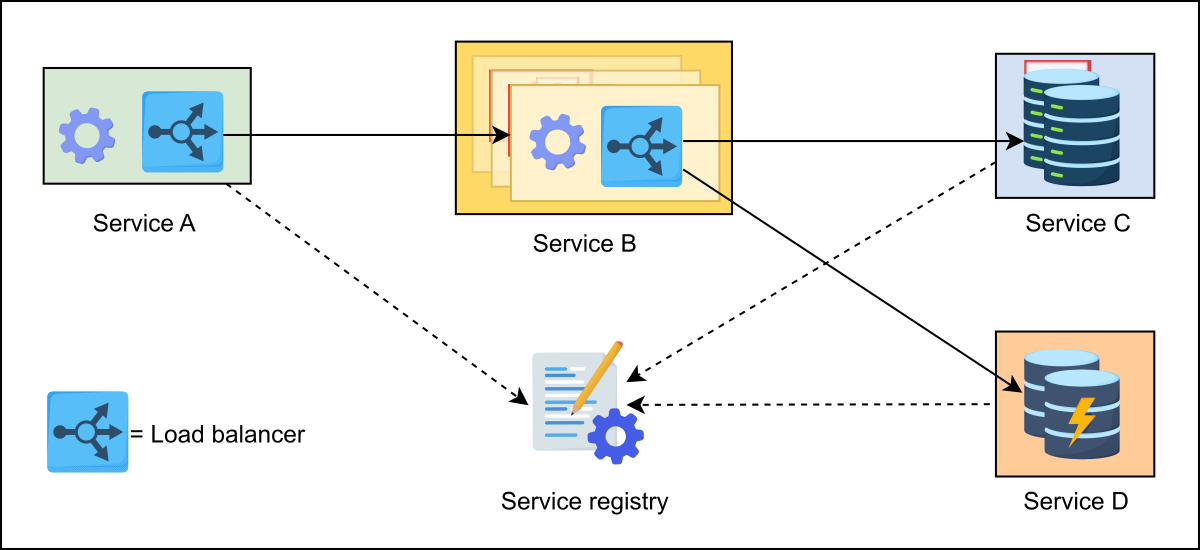
\includegraphics[width=0.5\textwidth]{Images/chapter_31/section_5379128533975040/4580163368386560.png}
 \caption{How client-side load balancing works}
\end{figure}

In the diagram above, Service A has to choose a relatively less-burdened instance of Service B. Therefore, it will make use of the load balancer component inside it to choose the most suitable instance of Service B. Using the same client-side load balancing method, Service B will talk to other services. It 's clear that Service A is the client when it is calling Service B, whereas Service B is the client when it is talking to Service C and D. As a result, there will be no central entity doing load balancing. Instead, every node will do load balancing of its own.
\\
\textbf{Advantages}: Using client-side load-balancing has the following benefits.

\begin{itemize}
\item
\protect\phantomsection\label{lZWCl4z9hi_xwd3Q5v0lv}
Less hardware infrastructure/layers are required to do load balancing.
\item
\protect\phantomsection\label{OWLXIO-1srmUK_wbwMVo_}
Network latency will be reduced because of no intermediate hop.
\item
\protect\phantomsection\label{MuY1CRR6dfX4XDZmAHSJQ}
Client-side load balancers eliminate bandwidth bottlenecks. On the other hand, in a dedicated load balancing layer, all requests go through a single machine that can choke if traffic multiplies.
\item
\protect\phantomsection\label{8UAqtNbQKrXpg4egeccc3}
Fewer points of failure in the overall system.
\item
\protect\phantomsection\label{KZTkHRDMcfMbsf4Zo71_X}
There is no end users queue waiting for the resource (server) for the particular services because many load balancers are routing the traffic. Eventually , it increases the quality of experience (QoE).
\end{itemize}
\\
Many real-world applications like Twitter, Yelp, Netflix, and others use client-side load balancing. We 'll discuss the client-side load balancing techniques used by Twitter in the next section.

\subsection{Client-side load balancing in Twitter}\label{_bZdMkVP1-uC4QF8Xx3Ax}
\\
Twitter uses a client-side load balancer referred to as \textbf{deterministic} \textbf{aperture}(Aperture specifies the number of sessions to be made with the calling service.) that is part of a larger RPC framework called Finagle. \textbf{Finagle} is a protocol-agnostic(Protocol-agnostic systems are protocol-independent such that it enables the communication between a variety of protocols.), open-source, and asynchronous RPC library.
\begin{quote}
\textbf{Note:} Consider the following question. What does the client-side load balancer of Twitter balance on? That is, what parameters are used to fairly balance the load across different servers?
\end{quote}
\\
Twitter primarily uses two distributions to measure the effectiveness of a load balancer:

\begin{enumerate}
\item
\protect\phantomsection\label{xY0D0QHR2BqcEEsIBPTmR}
The distribution of requests (OSI layer 7)
\item
\protect\phantomsection\label{SZ1Rxw5CHUkMizXU8mZmG}
The distribution of sessions (OSI layer 5)
\end{enumerate}
\\
Although requests are the key metric, sessions are an important attribute for achieving a fair distribution. Therefore, we'll develop techniques for fair distribution of requests as well as sessions. Let 's start with the simple technique of Power of Two Random Choices (P2C) for request distribution first.

\subsubsection{Request distribution using P2C}\label{lwfRS95L7HGNy0GzhIz1N}
\\
The \textbf{P2C technique} for request distribution gives uniform request distribution as long as sessions are uniformly distributed. In P2C, the system randomly picks two unique instances (servers) against each request, and selects the one with the least amount of load. Let's look at the illustration below to understand P2C.

\begin{figure}[htbp]
 \centering
 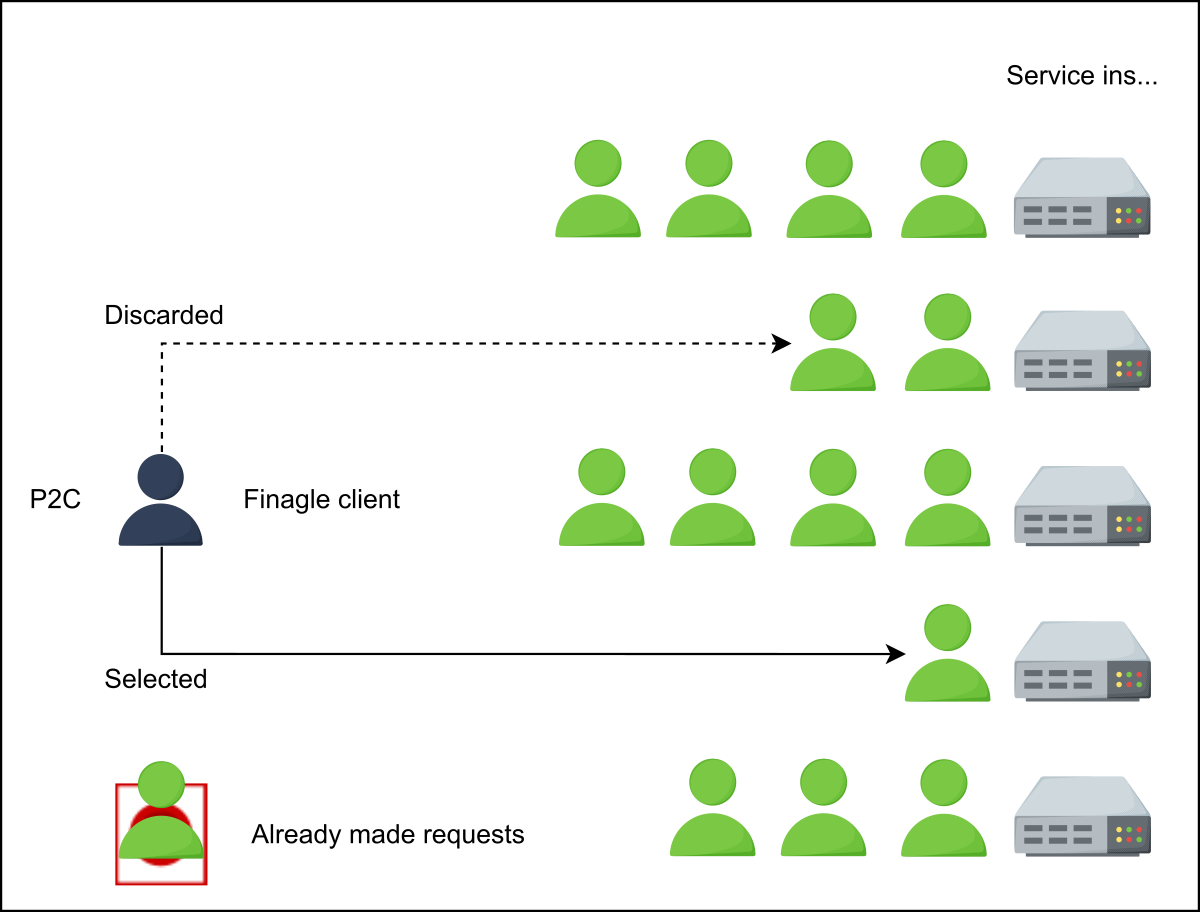
\includegraphics[width=0.5\textwidth]{Images/chapter_31/section_5379128533975040/4597503754633216.png}
 \caption{Power of two random choices}
\end{figure}

P2C is based on the simple idea(See ``The power of two choices in randomized load balancing'' by M. Mitzenmacher .) that comparison between two randomly selected nodes provides load distribution that is exponentially better than random selection
\\
Now that we've established how to distribute requests fairly, let's explore different techniques of session distribution.

\subsubsection{Session distribution}\label{HwcD4lxVOZRNbgR9TLvKf}
\\
\textbf{Solution 1}: We'll start our discussion with the \textbf{Mesh topology}. Using this approach, each client (load balancer) starts a session with all of the given instances of a service. The illustration below represents the concept of mesh topology.

\begin{figure}[htbp]
 \centering
 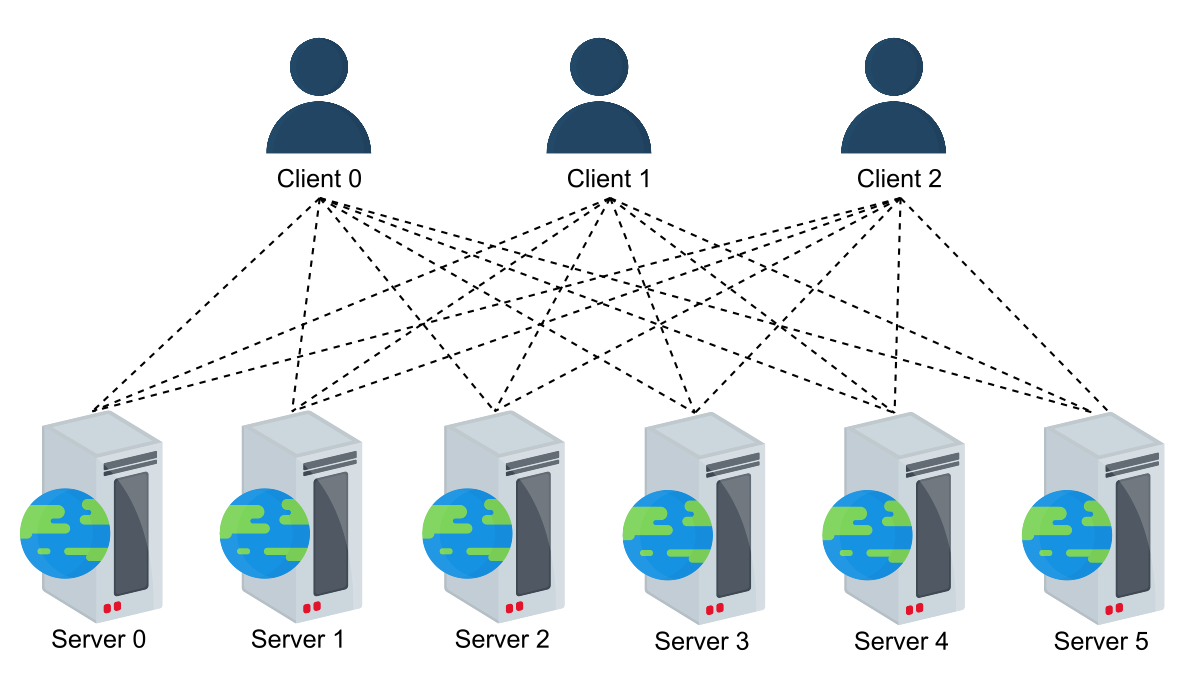
\includegraphics[width=0.5\textwidth]{Images/chapter_31/section_5379128533975040/6660028501852160.png}
 \caption{Mesh topology}
\end{figure}

Obviously, this method is fair because the sessions are evenly distributed. However, the even distribution of sessions comes at a very high cost, especially when scaled to thousands of servers. Apart from that, some unhealthy or stale sessions may lead to failures.
\\
\textbf{Solution 2}: To solve the problem of scalability with solution 1, Twitter devised another solution called \textbf{random aperture}. This technique randomly chooses a subset of servers for session establishment.

\begin{figure}[htbp]
 \centering
 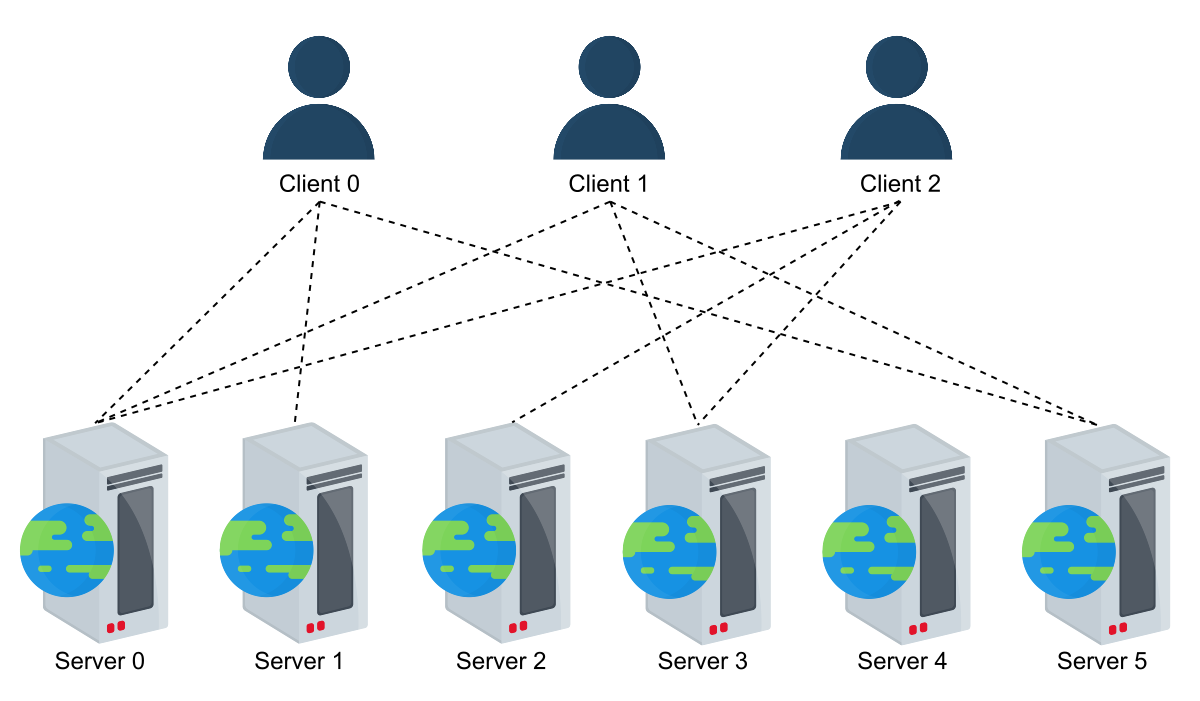
\includegraphics[width=0.5\textwidth]{Images/chapter_31/section_5379128533975040/5096629795553280.png}
 \caption{Random aperture}
\end{figure}

Of course, random selection will reduce the number of established sessions as we can see in the diagram above. However, the question is, how many servers will be chosen randomly? This is not an easy question to answer and the answer varies, depending on the request concurrency of a client.
\\
To answer the question above, Twitter installed a \textbf{feedback controller} inside the random aperture that decides the subset size based on the client's load. As a result, we're able to reduce the session load and ensure scalability. However, this solution isn't fair. We can see the imbalance in the illustration above such that \textbf{Server 4} has no session whereas \textbf{Server 0} has three sessions.
\\
This imbalance creates problems such as idle servers, high load on a few servers, and so on. Therefore, we need a solution that is both fair and scalable.
\\
\textbf{Solution 3}: We learned from solution 2 that we can scale by subsetting the number of session establishments. However, we failed to do the session distribution fairly. To resolve the problem, Twitter came up with a \textbf{deterministic aperture} solution. The key benefits of this approach are:

\begin{itemize}
\item
\protect\phantomsection\label{_3_QqEj6_G3BR2qts9sS7}
Little coordination is required between clients and servers to converge on a solution.
\item
\protect\phantomsection\label{E6svdNrN4IRXkBNeUrz35}
Minimal disruption occurs if there are any changes in the number of clients or server instances for whatever reason.
\end{itemize}
\\
For this solution, we represent clients and servers in a ring with equally distanced intervals, where each object on the ring represents the node or server labeled with a number. The illustration below shows what Twitter refers to as the discrete ring coordinates (that is, a specific point on the ring).

\begin{figure}[htbp]
 \centering
 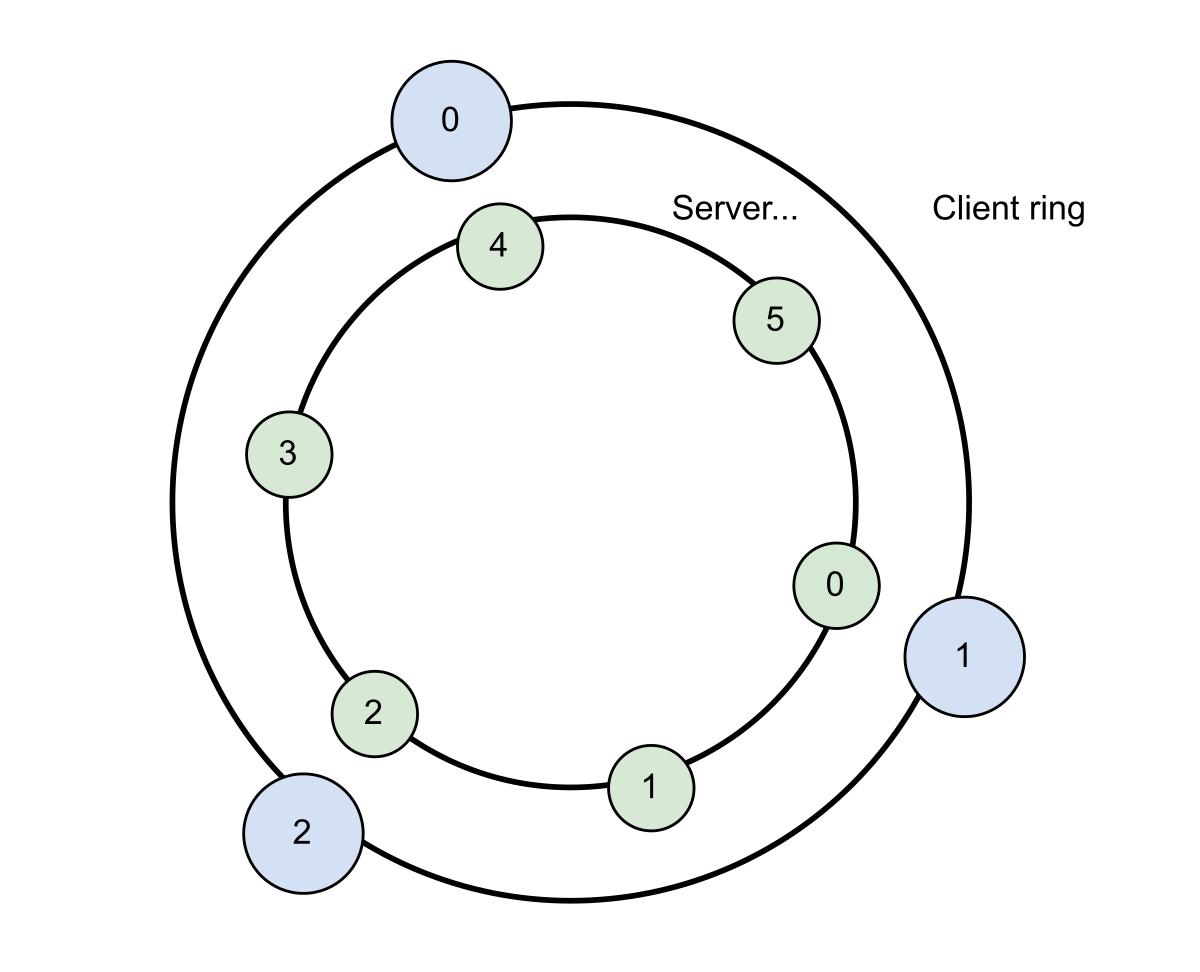
\includegraphics[width=0.25\textwidth]{Images/chapter_31/section_5379128533975040/6054097392500736.png}
 \caption{Ring coordinates}
\end{figure}

Now, we compose client and server rings to derive a relationship between them. We
\textquotesingle ve also defined an aperture size of 3. Each client will create a session with three servers in the ring. Clients select a server by circulating clockwise in the ring. This approach is similar to consistent hashing, except that here we guarantee equal distribution of servers across the ring. Let
\textquotesingle s see the illustration below where clients have sessions with servers chosen from the given list of servers, respectively.

\begin{figure}[htbp]
 \centering
 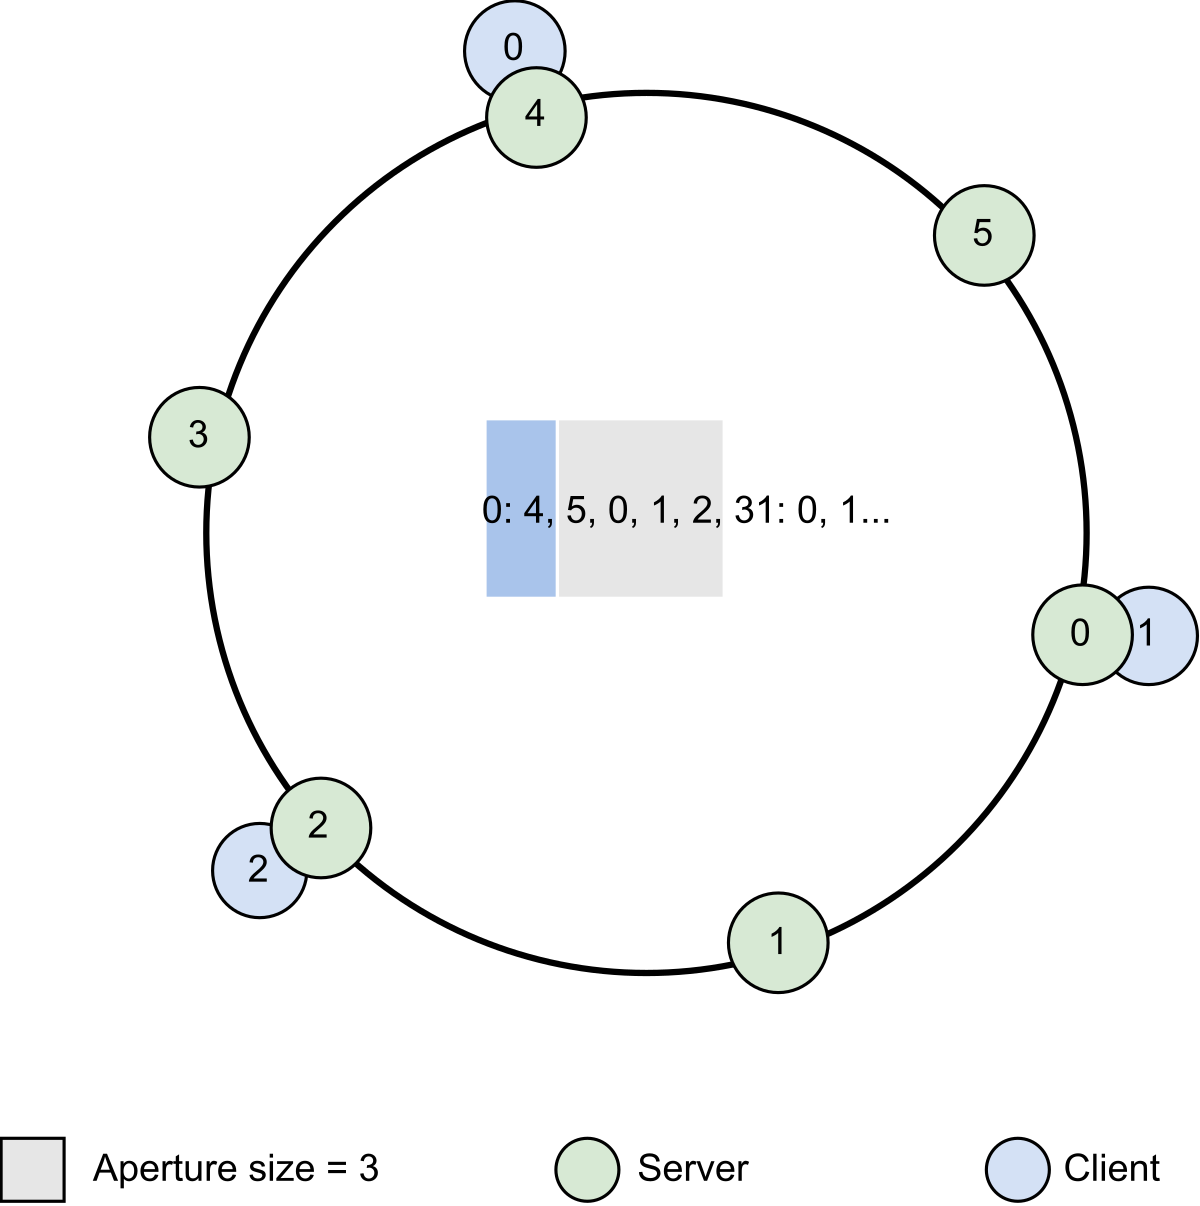
\includegraphics[width=0.25\textwidth]{Images/chapter_31/section_5379128533975040/5655305686089728.png}
 \caption{Merge client and server ring coordinates}
\end{figure}

In the diagram above, client 0 establishes sessions with servers 4, 5, and 0. Client 1 establishes sessions with servers 0, 1, and 2, whereas Client 2 establishes sessions with servers 2, 3, and 4. When the aperture rotates or moves in the given subset of arrays of the same size, each client\textquotesingle s service has new servers available to create sessions. The number of sessions established per server is shown in the figure below.\\

\begin{figure}[htbp]
 \centering
 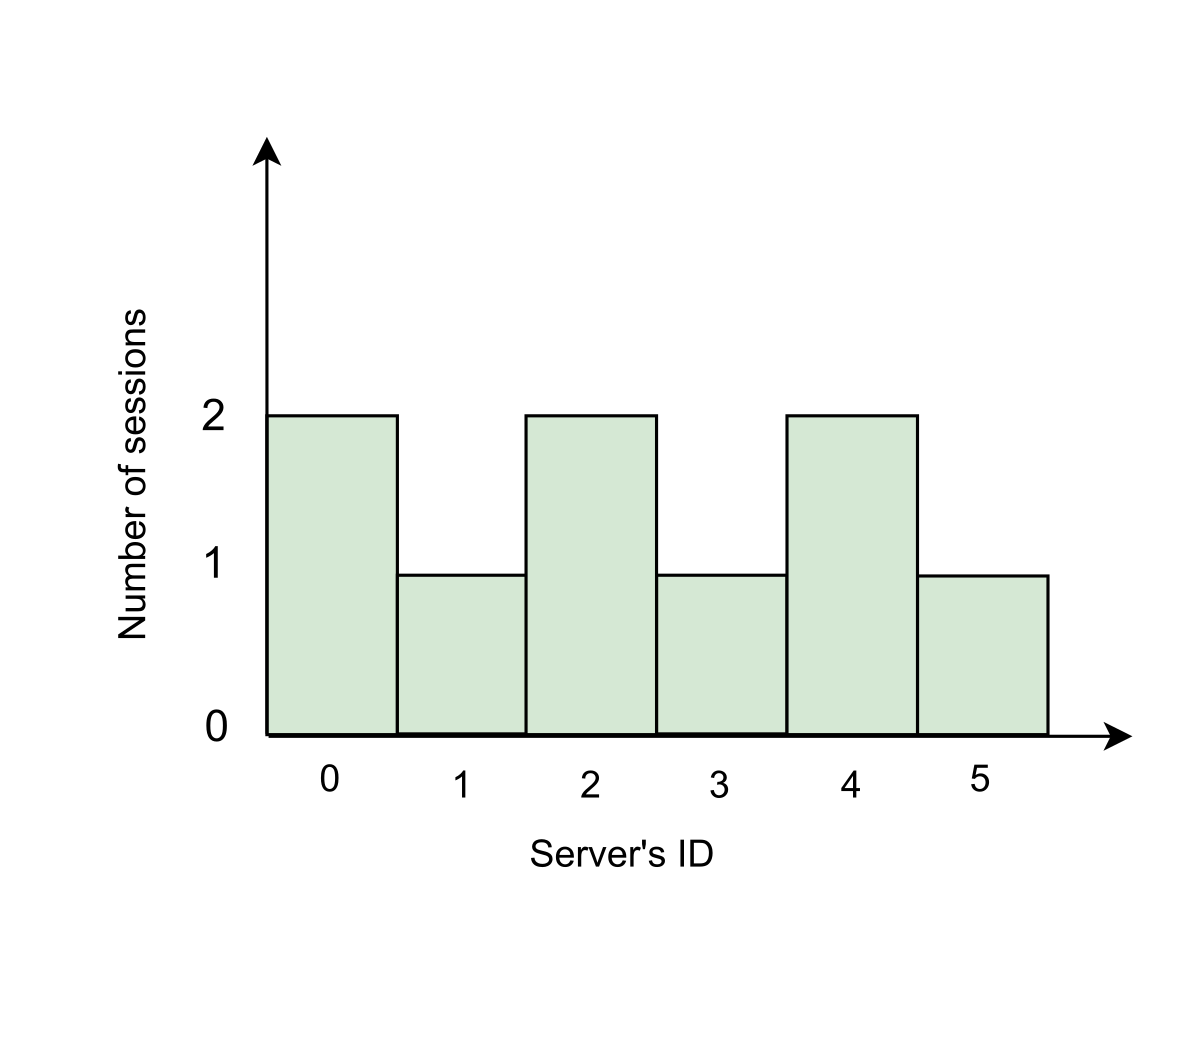
\includegraphics[width=0.25\textwidth]{Images/chapter_31/section_5379128533975040/6641692295299072.png}
 \caption{Number of sessions established per server}
\end{figure}

We can see that there\textquotesingle s no idle server or server with a high load in the histogram graph above. Thus , we achieved a fair distribution for the clients belonging to the same service. It
\textquotesingle s clear that we\textquotesingle ve half resolved the problem by improving the session distribution among servers as compared to the random aperture (solution 02). However, the problem of unfair distribution can escalate as the number of clients grows. In that case, some servers will get crowded when more than one client (service) talks to the back-end servers. Let
\textquotesingle s see the illustration below to understand the problem.

\begin{figure}[htbp]
 \centering
 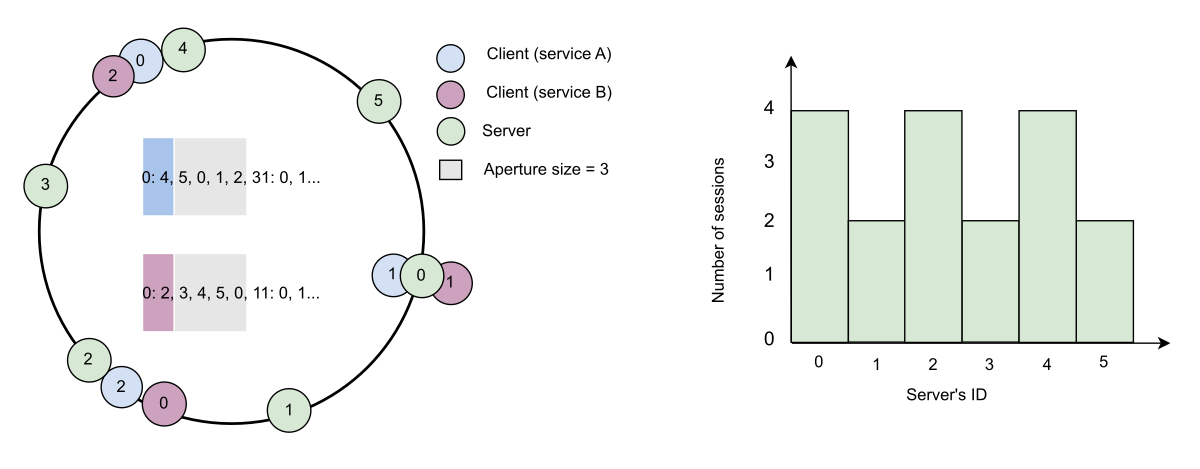
\includegraphics[width=0.5\textwidth]{Images/chapter_31/section_5379128533975040/5905463170564096.png}
 \caption{Two different clients creating session with backend servers}
\end{figure}

The illustration above depicts that the problem compounded as we increased the number of clients (services). The solution is continuous ring coordinates where we derive relationships between clients and servers using overlapping ring slices, rather than specific points on the rings. The important thing here is that the overlapping of rings can be partial since servers on the ring may not have enough instances to divide among the clients equally. Let
\textquotesingle s look at the illustration below.

\begin{figure}[htbp]
 \centering
 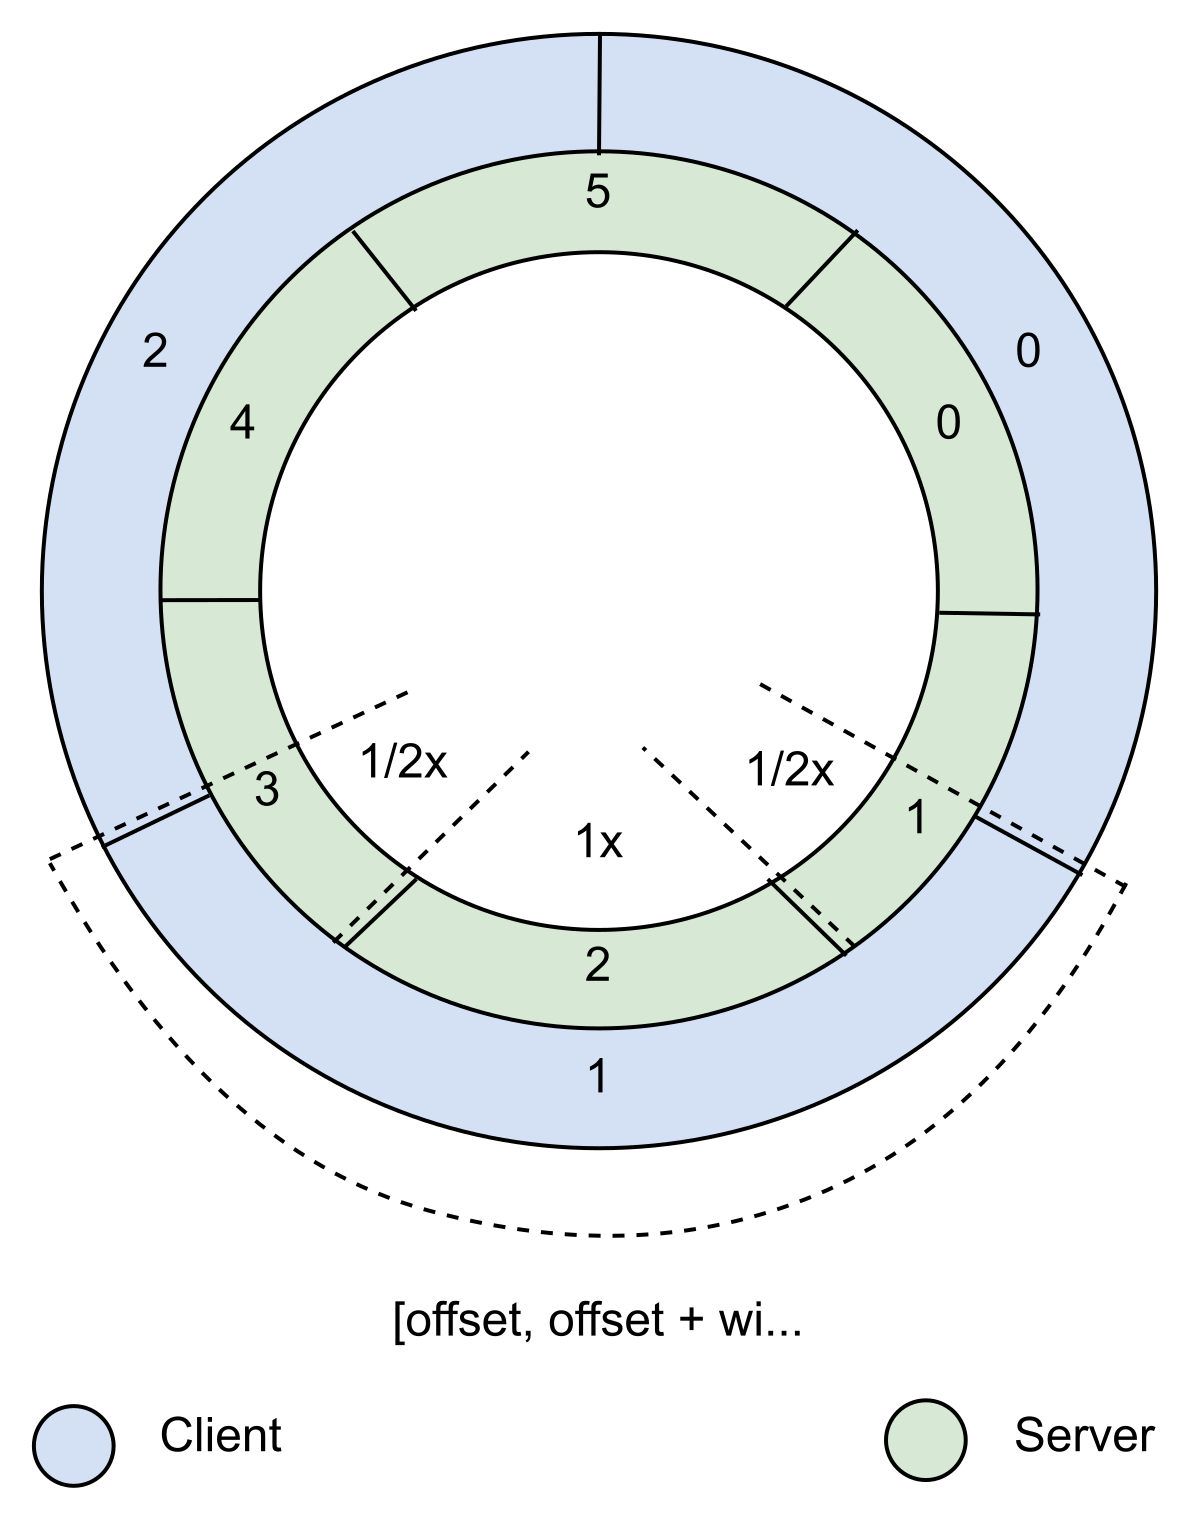
\includegraphics[width=0.25\textwidth]{Images/chapter_31/section_5379128533975040/5169676384731136.png}
 \caption{Overlapping among clients' services and servers}
\end{figure}

The illustration above shows that clients 0 and 1 (symmetrically) share the same server (server 1). It means that there is fractional overlapping concerning the ring coordinates. However, this overlapping can lead to asymmetric sharing as well. Symmetric or asymmetric, the load balancing can be done through P2C. For instance, in the diagram above, servers 1 and 3 will receive half the load that server 2 gets. This means that a server can receive more or less load, depending on its overlapped slice size with a client.
\\
Now, we know how to map clients to the subset of the servers. We'll use P2C with continuous ring coordinates. The client will pick points (coordinations) in its range instead of picking the instance of the server. The selection process of clients to create sessions with backend servers are as follows:

\begin{enumerate}
\item
\protect\phantomsection\label{NRp7HvXxupcuJKYj2r8CG}
Pick two coordinates (offset, offset + width) within its range and map these coordinates to the discrete instances (servers).
\item
\protect\phantomsection\label{9LqPABod8NJIr2oIsGxA3}
Select the one instance with the most negligible load from two chosen instances (P2C) by its degree of intersection.
\end{enumerate}
\begin{quote}
\textbf{Note:} Continuous aperture is scalable and fair at the cost of an additional session over boundary node due to partial overlapping. It is also able to achieve little coordination and minimal disruption.
\end{quote}
\\
Let's look at the below table to get an overview of the discussed approaches.

\textbf{Summary of Solutions for Session Distribution}

\begin{table}[htbp]
\centering
\small
\adjustbox{max width=\textwidth}{
\begin{tabular}{|p{0.309\textwidth}|p{0.214\textwidth}|p{0.218\textwidth}|p{0.209\textwidth}|}
\hline
\textbf{Approach} & \textbf{Scalability} & \textbf{Fair distribution} & \textbf{Cost effectiveness} \\
\hline
\hline
\textbf{Mesh topology} & \textbf{no} & \textbf{yes} & \textbf{no} \\
\hline
\textbf{Random aperture} & \textbf{yes} & \textbf{no} & \textbf{yes} \\
\hline
\textbf{Deterministic aperture} \textbf{(discrete ring)} & \textbf{yes} & \textbf{weak} & \textbf{yes} \\
\hline
\textbf{Deterministic aperture} \textbf{(continuous ring)} & \textbf{yes} & \textbf{yes} & \textbf{yes} \\
\hline
\end{tabular}
}
\caption{Summary of Solutions for Session Distribution}
\end{table}

Can you describe a real-world scenario where a client-side load-balancing approach would offer significant advantages over other load-balancing methods? Justify your answer with reasoning.

\subsection{Conclusion}\label{s3KVLv7uyu4OWptmF3DNu}
\\
This design problem highlights that tweaking the performance of common building blocks and utilizing the right (rich) combination of them is necessary for real-world services. Our needs from one service to the next will dictate which design point we choose in our solution space. In this chapter, we saw examples of how Twitter uses a combination of data stores and custom algorithms for load-balancing.

% End of section content